\documentclass[12pt]{article}
\usepackage[spanish]{babel}
\usepackage[utf8]{inputenc}
\usepackage{amsmath}
\usepackage{geometry}
\usepackage{tcolorbox}
\usepackage{graphicx}

\geometry{margin=2.5cm}


\title{FACULTAD DE INGENIERÍAS Y ARQUITECTURA\\
ESCUELA PROFESIONAL DE INGENIERÍA DE SOFTWARE}

\author{}
\date{}

\begin{document}

\maketitle


    \centering
    \includegraphics[width=0.5\textwidth]{logo_web.jpg}
   
   \section*{COMPILADORES}
   
    \section*{Integrantes}
    Johan Leonardo Marquez Zúñiga \\
    Diego Paolo Nova Rosas\\ 
    Angelica Valeria Castillo Tovar\\
    Renzo Josue Murrillo Alvarez
    \label{fig:mi_imagen}
\end{figure}
\newpage


\section*{Introducción}
\section*{Motivación}

 Ofrecer una sintaxis simple pero estructurada que permita identificar de forma clara las construcciones fundamentales de un lenguaje de programación. Como funciones, estructuras de control, asignaciones y expresiones.

Nuestro lenguaje se inspira en lenguajes de alto nivel como Python y C, pero con una notación simplificada y un conjunto reducido de tokens. Esto permite centrarse en el análisis léxico y sintáctico, así como en la construcción del árbol de derivación para su posterior visualización o análisis semántico.



\section*{Descripción}


\begin{alltt}
\section*{Sentencias(S)}
   - Una declaración (DECLARACION)\\ 
   - Una secuencia de sentencias (\textbf{S} &\rightarrow \textbf{S})\\
   - Vacía (\textbf{S} &\rightarrow \textbf{\epsilon \\})
\end{alltt}

Esto permite que las declaraciones se agrupen o se definan de forma individual.\\\\


\section*{Declaraciones(Declaración)}
   - Un símbolo especial: (\#\))\\\\ 
   - Un identificador (id) usado como nombre de variable\\
   - Una declaración extendida (DECL EXTRA), que permite asignaciones

\section*{Declaraciones extendidas(DECL EXTRA)}
   - Un operador de asignación (=)\\
   - Una expresion (E)\\

\section*{Expresiones(E)}
   - Un término(T) que puede ser un id o un número(\#\))
   
   - Una continuación de expresión (E') que permite encadenar operadores\\
   
\section*{Extensión de expresiones(E')}
\end{alltt}
Sirve para definir operaciones aritméticas:\\

   - Un operador como el(+)\\
   
   - Un nuevo término (T)\\
   - Otra extensión (E') o el fin de la expresión (\epsilon)\\

\section*{Operadores(OPER)}
\end{alltt}
    - Solo se define el operador de suma (+), lo cual restringe las operaciones posibles.

\section*{Especificación léxica}
A continuación, se listan los tokens utilizados por el analizador léxico, con sus respectivas expresiones regulares:

\begin{center}
\renewcommand{\arraystretch}{1.2}
\begin{tabular}{|l|l|p{7cm}|}
\hline
\textbf{Token} & \textbf{Expresión Regular} & \textbf{Descripción} \\
\hline
\texttt{FUNK\_RET} & \verb|funk_ret| & Define una función que retorna un valor. \\
\texttt{FUNK\_NOT\_RET} & \verb|funk_not_ret| & Define una función que no retorna valor. \\
\texttt{RET} & \verb|ret| & Palabra reservada para retornar un valor desde una función. \\
\texttt{IF} & \verb|if| & Estructura condicional: ejecuta un bloque si se cumple la condición. \\
\texttt{ELSE} & \verb|else| & Alternativa del \texttt{if} si la condición es falsa. \\
\texttt{WHILE} & \verb|while| & Bucle que se ejecuta mientras se cumpla una condición. \\
\texttt{FOR} & \verb|for| & Bucle con inicialización, condición y actualización. \\
\texttt{IGUAL} & \verb|=| & Operador de asignación de valores a variables. \\
\texttt{ADD} & \verb|+| & Operador de suma aritmética. \\
\texttt{LESS} & \verb|-| & Operador de resta aritmética. \\
\texttt{MULT} & \verb|*| & Operador de multiplicación. \\
\texttt{DIV} & \verb|/| & Operador de división. \\
\texttt{MENOR\_IGUAL} & \verb|<=| & Operador de comparación: menor o igual que. \\
\texttt{MAYOR\_IGUAL} & \verb|>=| & Operador de comparación: mayor o igual que. \\
\texttt{DIFERENTE} & \verb|<>| & Operador de comparación: distinto. \\
\texttt{IGUAL\_QUE} & \verb|==| & Operador de comparación: igualdad. \\
\texttt{MENOR} & \verb|<| & Operador de comparación: menor que. \\
\texttt{MAYOR} & \verb|>| & Operador de comparación: mayor que. \\
\texttt{AND} & \verb|@| & Operador lógico AND. \\
\texttt{OR} & \verb|//| & Operador lógico OR. \\
\texttt{LEFT\_PAR} & \verb|(| & Paréntesis izquierdo, usado para agrupar expresiones. \\
\texttt{RIGHT\_PAR} & \verb|)| & Paréntesis derecho. \\
\texttt{INICIO} & \verb|{| & Delimita el inicio de un bloque de código. \\
\texttt{FIN} & \verb|}| & Delimita el fin de un bloque de código. \\
\texttt{COMA} & \verb|,| & Separa elementos, como parámetros en funciones. \\
\texttt{DECLARACION DE VARIABLE} & \verb|#| & Simboliza una declaración de variable. \\
\texttt{NUM} & \verb|num| & Representa un número entero o real. \\
\texttt{ID} & \verb|id| & Representa un identificador, como nombres de variables o funciones. \\
\texttt{WHITESPACE} & \verb|\s+| & Espacios en blanco; se ignoran en el análisis léxico. \\
\hline
\end{tabular}
\end{center}

\section*{Gramática Original}
\textbf{S} &\rightarrow \textbf{DECLARACION}\ \textbf{S} \\
\textbf{S} &\rightarrow \textbf{FUNCION}\ \textbf{S} \\
\textbf{S} &\rightarrow \textbf{CICLO}\ \textbf{S} \\
\textbf{S} &\rightarrow \textbf{IF}\ \textbf{ELSE}\ \textbf{S} \\
\textbf{S} &\rightarrow \textbf{E}\ \textbf{S} \\
\textbf{S} &\rightarrow \epsilon \\
\\
\textbf{DECLARACION} &\rightarrow \#\ id\ \textbf{DECL\_EXTRA} \\
\textbf{DECL\_EXTRA} &\rightarrow =\ \textbf{E} \\
\textbf{DECL\_EXTRA} &\rightarrow \epsilon \\
\\
\textbf{FUNCION} &\rightarrow \textbf{FUNK\_RET} \\
\textbf{FUNCION} &\rightarrow \textbf{FUNK\_NOT\_RET} \\
\\
\textbf{FUNK\_RET} &\rightarrow \text{funk\_ret}( \textbf{PARAMS} ) \{ \textbf{INSTRUCCIONES}\ \text{ret}\ \textbf{E} \} \\
\textbf{FUNK\_NOT\_RET} &\rightarrow \text{funk\_not\_ret}( \textbf{PARAMS} ) \{ \textbf{INSTRUCCIONES} \} \\
\\
\textbf{PARAMS} &\rightarrow id\ \textbf{PARAMS'} \\
\textbf{PARAMS'} &\rightarrow ,\ id\ \textbf{PARAMS'} \\
\textbf{PARAMS'} &\rightarrow \epsilon \\
\\
\textbf{INSTRUCCIONES} &\rightarrow \textbf{SENTENCIA}\ \textbf{INSTRUCCIONES} \\
\textbf{INSTRUCCIONES} &\rightarrow \epsilon \\
\\
\textbf{ASIGNACION} &\rightarrow id\ =\ \textbf{E} \\
\\
\textbf{SENTENCIA} &\rightarrow \textbf{DECLARACION} \\
\textbf{SENTENCIA} &\rightarrow \textbf{FUNCION} \\
\textbf{SENTENCIA} &\rightarrow \textbf{IF}\ \textbf{ELSE} \\
\textbf{SENTENCIA} &\rightarrow \textbf{CICLO} \\
\textbf{SENTENCIA} &\rightarrow \textbf{ASIGNACION} \\
\\
\textbf{IF} &\rightarrow \text{if} ( \textbf{A} ) \{ \textbf{INSTRUCCIONES} \} \\
\textbf{ELSE} &\rightarrow \text{else} \{ \textbf{INSTRUCCIONES} \} \\
\textbf{ELSE} &\rightarrow \epsilon \\
\\
\textbf{CICLO} &\rightarrow \textbf{WHILE} \\
\textbf{CICLO} &\rightarrow \textbf{FOR} \\
\\
\textbf{WHILE} &\rightarrow \text{while} ( \textbf{A} ) \{ \textbf{INSTRUCCIONES} \} \\
\textbf{FOR} &\rightarrow \text{for} ( \textbf{DECLARACION},\ \textbf{A},\ \textbf{E} ) \{ \textbf{INSTRUCCIONES} \} \\
\\
\textbf{A} &\rightarrow id\ \textbf{COMP}\ id\ \textbf{A'} \\
\textbf{A'} &\rightarrow \textbf{LOGICO}\ id\ \textbf{COMP}\ id\ \textbf{A'} \\
\textbf{A'} &\rightarrow \epsilon \\
\\
\textbf{E} &\rightarrow \textbf{T}\ \textbf{E'} \\
\textbf{E'} &\rightarrow \textbf{OPER}\ \textbf{T}\ \textbf{E'} \\
\textbf{E'} &\rightarrow \epsilon \\
\\
\textbf{T} &\rightarrow ( \textbf{E} ) \\
\textbf{T} &\rightarrow id \\
\textbf{T} &\rightarrow num \\
\\
\textbf{COMP} &\rightarrow <\ |\ >\ |\ <=\ |\ >=\ |\ <>\ |\ == \\
\textbf{LOGICO} &\rightarrow @\ |\ // \\
\textbf{OPER} &\rightarrow +\ |\ -\ |\ *\ |\ / \\
\end{lstlisting}


\section*{Lecturas aceptadas}
\begin{document}

\renewcommand{\arraystretch}{2} 
\setlength{\tabcolsep}{10pt}     

\begin{longtable}{
\hline
\texttt{
funk\_ret( id ) \{ \# id = id if( id < id ) \{ \# id \} ret id \}%
} \\[1.5ex] \hline

\texttt{%
funk\_not\_ret( id ) \{ \# id = id funk\_not\_ret( id ) \{ if ( id < id ) \{ \# id = num \} \# id = id + id \} \}%
} \\[1.5ex] \hline

\texttt{%
for ( \# id , id < id , id + num ) \{ for ( \# id , id <> id , id + num ) \{ \# id = num + id \} if ( id > id ) \{ \# id = ( id + num ) * id funk\_not\_ret ( id ) \{ while ( id < id ) \{ id = num + num \} \} \} \# id = num \}%
} \\[1.5ex] \hline

\texttt{%
funk\_not\_ret ( id ) \{ \# id = id funk\_not\_ret ( id ) \{ for ( \# id , id < id , id + num ) \{ \# id = num \} \# id = id + id \} \}%
} \\[1.5ex] \hline

\texttt{%
if ( id < id @ id < id ) \{ \# id = num + id \}%
} \\[1.5ex] \hline

\texttt{%
if ( id < id @ id < id ) \{ \# id = num + id \}%
} \\[1.5ex] \hline

\end{longtable}

\section*{Lecturas no aceptadas}

\begin{longtable}{
\hline
\texttt{if ( id < id id < id ) \{ \# id = num + id \}} \\
En esta parte quitamos el símbolo \texttt{@ and} para verificar que manda error. \\
\hline

\texttt{for ( ) \{ for ( \# id , id <> id , id + num ) \{ \# id = num + id \} if ( id > id ) \{ \# id = ( id + num ) * id funk\_not\_ret ( id ) \{ while ( id < id ) \{ id = num + num \} \} \} \# id = num \}} \\
El primer \texttt{for} no tiene parámetros, y la gramática requiere parámetros en la estructura del ciclo. \\
\hline

\texttt{funk\_n*ot\_ret ( id ) \{ \# id = id funk\_not\_ret ( id ) \{ for ( \# id , id < id , id + num ) \{ \# id = num \} \# id = id + id \} ret id \}} \\
Al final se agregó \texttt{ret id}, pero es un error ya que la función fue declarada como una función sin retorno (\texttt{funk\_not\_ret}). \\
\hline
\end{longtable}


\section*{Tabla sintáctica}
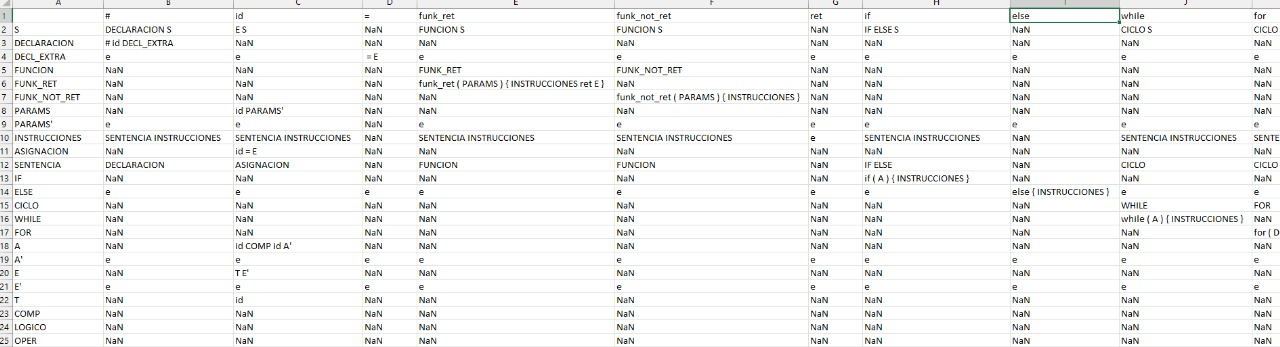
\includegraphics[width=1\textwidth]{tabla1.jpg}\\
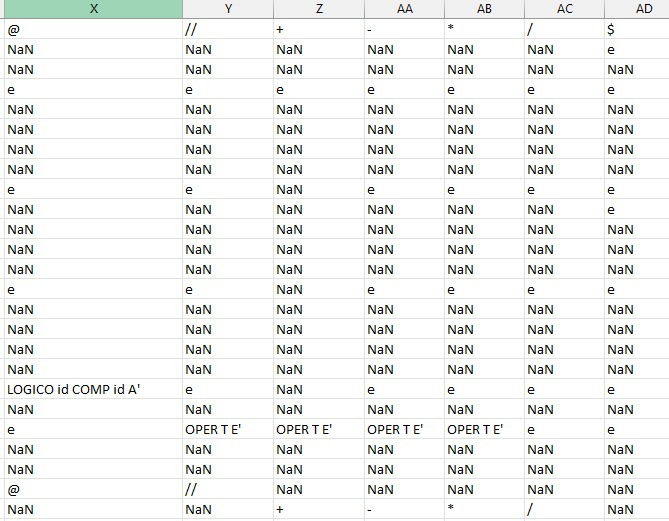
\includegraphics[width=1\textwidth]{tabla2.jpg}\\

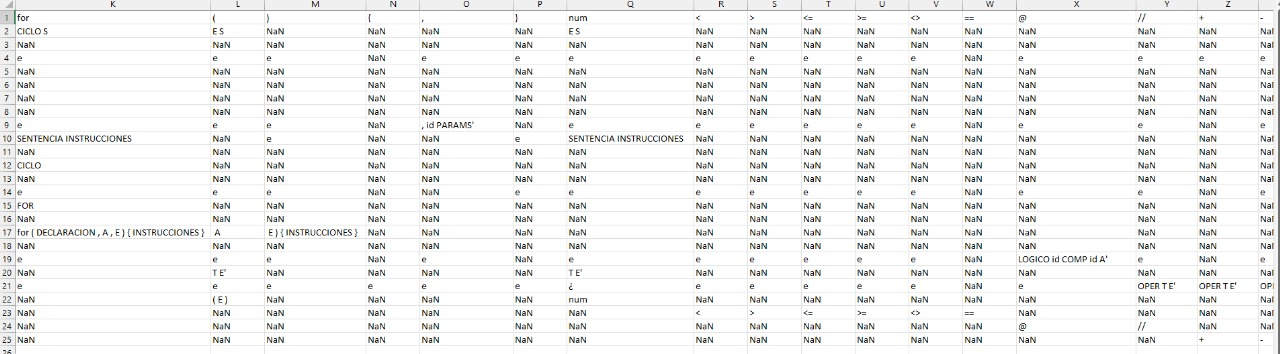
\includegraphics[width=1\textwidth]{tabla3.jpg}

\section*{Arbol}

Ejemplo de lectura:

\texttt{if ( id < id @ id < id ) \{ \# id = num + id \}}

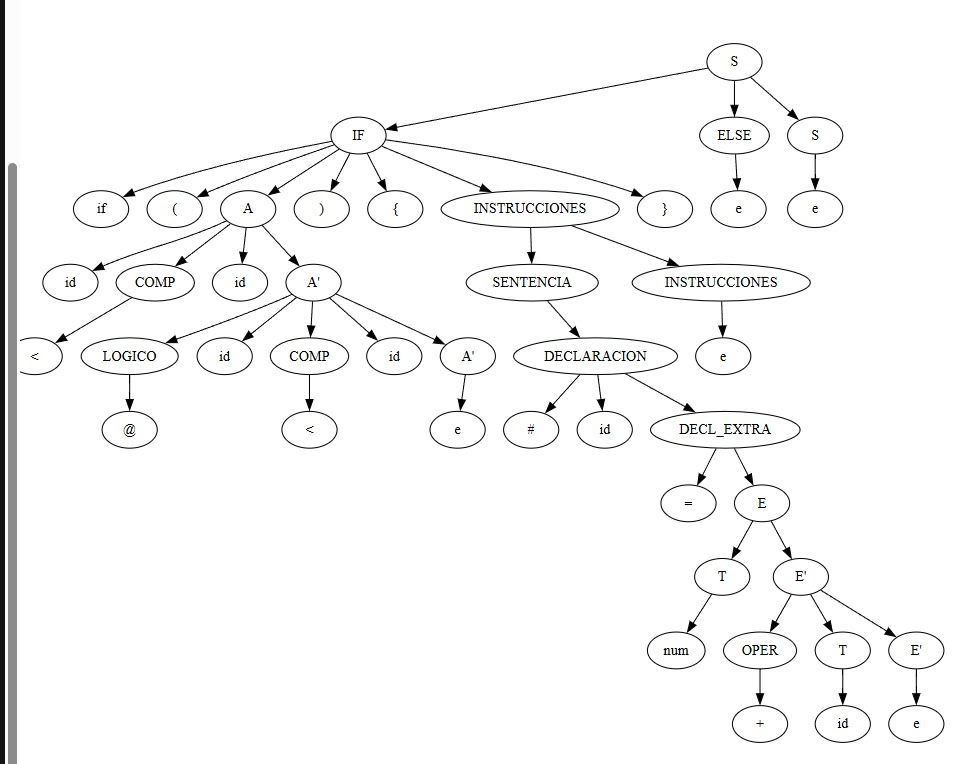
\includegraphics[width=1\textwidth]{arbol.jpg}










\end{document}

















































